\chapter{Теория}
\label{ch:intro}

Если подать на вход линейной цепи гармонический сигнал $x(t) = Acos(\omega_0t+\phi)$, то получим сигнал той же формы, но
амплитуда и фаза изменятся.

Запишем гармонический сигнал:

\[
x(t) = A \cos(\omega_0 t + \varphi)
\]

Если представить сигнал в комплексной форме, то гармонический сигнал $Acos(\omega_0t+\phi)$ - действительная часть такого сигнала:

\[
x(t) = \Re \{ A e^{i(\omega_0 t + \varphi)} \}
\]

Разложим экспоненту и получим комплексную амплитуду:

\[
\Re \{ A e^{i\varphi} e^{i\omega_0 t} \}
\]


\[
A e^{i\varphi} = A_k
\]

Итоговый сигнал будет иметь вид:

\[
x(t) = A_k e^{i\omega_0 t}
\]

Теперь пропустим сигнал через линейную цепь с импульсной характеристикой $h(\tau)$:

\[
y(t) = \int_{-\infty}^{\infty} h(t - \tau) x(\tau) d\tau = 
\int_{-\infty}^{\infty} h(t - \tau) A e^{i\omega_0 \tau} d\tau = 
\]

Поскольку $A e^{i\omega_0 t}$ не зависит от $\tau$, вынесем ее за знак интеграла. Заметим, что $A e^{i\omega_0 t}$ - наш исходный
сигнал $x(t)$. Под знаком интеграла можем увидеть ППФ над импульсной характеристикой, запишем этот интеграл как $H(iw)$.

\[
A e^{i\omega_0 t} \int_{-\infty}^{\infty} h(t - \tau) e^{-i\omega_0 t} d\tau =
A e^{i\omega_0 t} H(i\omega_0)
\]

\[
\boxed{H(i\omega) = \int_{-\infty}^{\infty} h(t) e^{-i\omega t} dt}
\]

ППФ от импульсной характеристики - комплексная частотная характеристика

\[
A_y = A_x \cdot H(i\omega_0)
\]

$
A_y = A_x \cdot H(i\omega_0) = |A_x| \cdot |H(i\omega_0)|
$ - комплексная амплитуда для гармонического сигнала на частоте $w_0$

Выходной сигнал цепи $y(t)$ будет отличаться только комплексной амплитудной.

\[
x(t) \leftrightarrow X(i\omega)
\]

\[
y(i\omega) = \boxed{X(i\omega) \cdot H(i\omega)}
\]

$H(iw_0)$ - комплексная коэффициент передачи 

\[
H(i\omega) = \frac{y(i\omega)}{x(i\omega)}
\]

\[
A(i\omega) = |H(i\omega)| e^{i\varphi(\omega)}
\]

Здесь $|H(i\omega)|$ - амплитудно-частотная характеристика (АЧХ), $e^{i\varphi(\omega)}$ - фазо-частотная характеристика (АЧХ). \\

Если импульсная характеристика RC цепи равна

\[
h(t) = \frac{1}{T}e^{-\frac{t}{T}}
\]

то комплексная частотная характеристика равна

\[
H(iw) = \frac{1}{1+T}
\]

АЧХ можно посчитать как

\[
|H(i\omega)| = \frac{1}{\sqrt{1 + (\omega RC)^2}}
\]

а ФЧХ как

\[
\varphi(\omega) = -\arctg(\omega RC)
\]

\section*{Пример}

Допустим, мы подали на вход системы $x(t) = Acos(\omega_0t)$ и получили следующие характеристики цепи:

\begin{figure}[H]
    \centering
    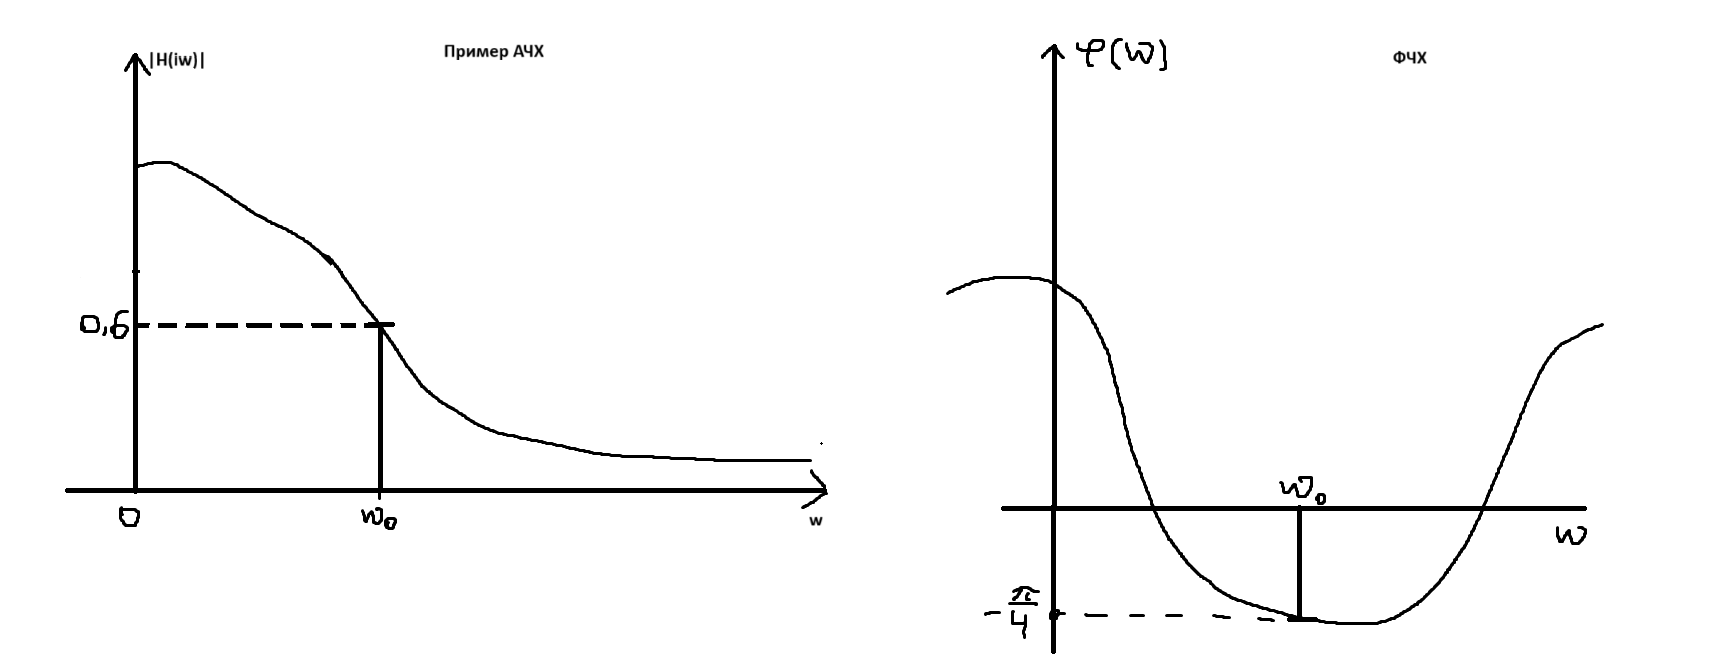
\includegraphics[width=1.0\textwidth]{afr.png}
    \caption{АЧХ и ФЧХ цепи}
\end{figure}

АЧХ и ФЧХ показывают, насколько хорошо или плохо цепь будет пропускать сигнал на определенных частотах. В нашем случае можем видеть,
что чем больше частота, тем ниже амплитуда выходного сигнала, т.е высокие частоты срезаются и остаются только низкие. \\

На выходе получим $y(t) = |H(i\omega_0)|cos(\omega_0)t-\phi(\omega_0) = 0.6cos(\omega_0t + \frac{\phi}{4})$ \\

Таким образом, зная АЧХ и ФЧХ цепи, мы можем расчитать выходной сигнал на конкретной частоте $\omega_0$.

\section*{Условие безыскаженной передачи сигналов}

При передаче сигналов через LTI цепь амплитуды и фазы спектральных составляющих сигналов будут изменяться в соответствии с формой
$H(i\omega)$, потому что АЧХ и ФЧХ изменяются неравномерно, что приведет к изменению формы сигнала на выходе. Условие отсутсвия искажений (изменения формы): \\

Чтобы передача была без искажений, нужно чтобы коэффициент усилениия $H_0$ не зависел от частоты (график константы), в таком случае
на каждой частоте сигнал будет принимать одинаковое значение и искажений не будет. Также необходимо, чтобы фаза линейно зависела 
от частоты, тогда фазовый сдвиг будет зависеть только от времени $t_0$. Все эти условия должны выполняться на частоте $\omega_1 <= \omega <= \omega_2$

$$\phi(\omega) = -\omega t_0$$ 
$$|H(i\omega)| = H_0$$ 

Идеальный выходной сигнал можно записать так:

$y(t)$ = $H_0x(t - t_0)$

\section*{Линейная цепь - частотно-селективный фильтр}

Основное применение линейных цепей - фильтрация сигналов. Линейная цепь пропускает определенные компоненты сигнала с 
минимальным подавлением и подавляет остальные компоненты. \\

Частота среза - частота, после которой сигнал начинает сильно ослабевать

$$\boxed{f_c = \frac{1}{2\pi RC}}$$

Если знать частоту среза, то можно определить участок, на котором искажения сигнала будут минимальны, т.е где АЧХ $\approx const$
и $\phi(\omega) = -\omega t_0$ \\

Идеальная АЧХ RC цепи:

\begin{figure}[H]
    \centering
    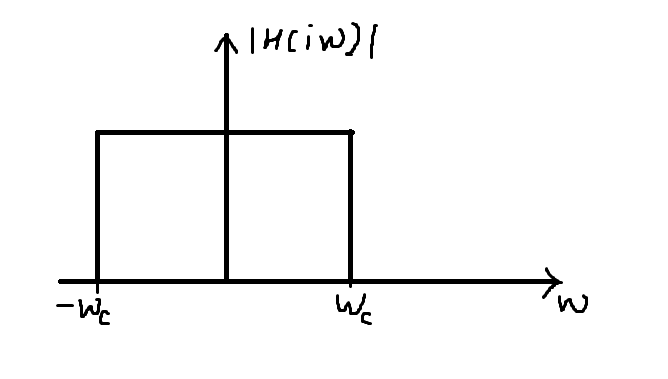
\includegraphics[width=1.0\textwidth]{ifafr.png}
    \caption{Идеальная АЧХ}
\end{figure}

Видим, что на промежутке $[-w_c;w_c]$ АЧХ никак не меняется. \\

Изобразим идеальную АЧХ ФНЧ (фильтра низкой частоты)

\begin{figure}[H]
    \centering
    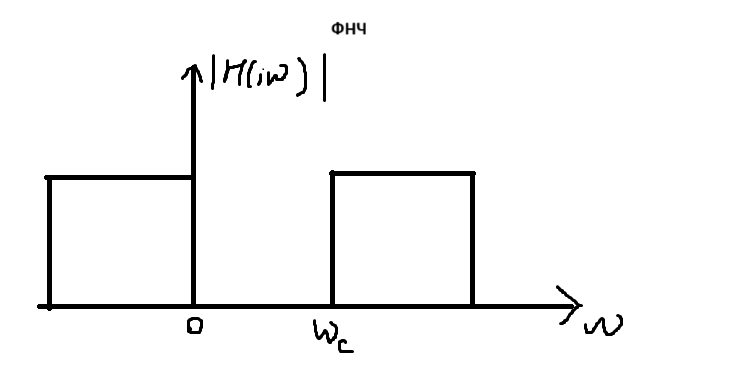
\includegraphics[width=1.0\textwidth]{fnch.png}
    \caption{Идеальная АЧХ ФНЧ} 
\end{figure}

Данная АЧХ является прямоугольным сигналом. Это значит, что импульсная характеристика такой цепи имеет вид $h(t) = \frac{sin\omega_ct}{\omega_ct}$.
Данная функция никогда не угаснет, т.е $-\infty <= t <= \infty$. Это значит, что реакция идеального фильтра бесконечна, т.е при подаче
сигнала на такой фильтр мы никогда не получим результа. Это всего лишь идеальная модель и в жизни такого не бывает, значит, 
АЧХ и ФЧХ фильтров не идеальны.



\endinput